\documentclass[a4paper, 11pt]{article}
\usepackage{comment} % enables the use of multi-line comments (\ifx \fi) 
\usepackage{graphicx}
\usepackage[utf8]{inputenc}
\usepackage[francais]{babel}
\usepackage[T1]{fontenc}
\usepackage{subfig}
\usepackage{fullpage} % changes the margin

\begin{document}
%Header-Make sure you update this information!!!!
\noindent
\large\textbf{Graphs \& Networks \- GogolCar Report} \hfill \textbf{Benjamin Bertrand} \\
\normalsize M1 ATAL, ORO \hfill Due Date: 30/11/2016 \\
F.S.T. de Nantes \hfill Prof. Irena Rusu\\


\section*{Problem Statement}
3 algorithmes de parcours de graphes, pour simuler le parcours d'une voiture
dans une ville. Les rues sont des arêtes non-oriente et peuvent parfois être
considérer comme deux arcs orientes. les rues sont délimité par des places, les
nœuds du graphe.

Pour ce projet, j'utilise les lambda java 8, ainsi que l'API Stream qui permet
de faire des opérations ensembliste intéressantes et simplifie grandement le
code.

\section{Mapper en listes d'adjacence}
\begin{verbatim}
Map<Square, List<Street>> adjacentStreet() {
    return getStreets().collect(
        toMap(
            st -> st.sq1, 
            st -> Stream.of(st).collect(toList()), 
            (list1, list2) -> Stream.concat(list1.stream(),list2.stream()).collect(toList())
        )); 
}
\end{verbatim}
On cherche par exemple a associer chaque sommet au rues qui lui sont adjacentes.
Pour cela, on prends la liste des rues, on extrait les sommets et les agrègent
selon les règles suivante.

\begin{itemize}
  \item On prend la clef de la map comme étant l'un des sommet de la rue (toujours le même sq1).
\begin{verbatim}
st -> st.sq1
\end{verbatim}

\item On prend la rue elle même comme valeur correspondant a la clef. Mais sous
forme de liste pour permettre l’agrégation.
\begin{verbatim}
st -> Stream.of(st).collect(toList())
\end{verbatim}

\item On définit la règles pour les cas ou la clef apparaît plusieurs fois, ici
une concaténation des collections.
\begin{verbatim}
(list1, list2) -> Stream.concat(list1.stream(),list2.stream())
                        .collect(toList())
\end{verbatim}
\end{itemize}


\section{Calcul du degré de chaque sommets}
En utilisant un Stream de Street on peut réduire le set entier en une
  valeur:
\begin{verbatim}
long nbDegreImpair() {	
    return getStreets()
                .flatMap(street -> Stream.of( street.sq1, street.sq2 ))
                .collect(toMap(s->s, s -> 1, Integer::sum))
                .entrySet()
                .stream()
                .filter(ent -> (ent.getValue().longValue() % 2) == 1)
                .count();
    }
\end{verbatim}
\begin{itemize}
  \item convertit une Street en un Stream de Square possédant toute les occurrences de
sommet comme extrémité d'une rue.
\begin{verbatim}
street -> Stream.of( street.sq1, street.sq2 )
\end{verbatim} 
  \item Map collector, on associe 1 a chaque sommet puis on les cumul par somme lorsque
le sommet apparaît plusieurs fois.
\begin{verbatim}
toMap(s->s, s -> 1, Integer::sum)  // Map<Square,Integer>
\end{verbatim}
  \item Pour chaque clef-valeur, On filtre les sommets impairs uniquement puis on
en compte la somme.
\begin{verbatim}
 .entrySet()  // Set<Entry<Square,Integer>>
 .stream()    // Stream<Entry<Square,Integer>>
 .filter(ent -> (ent.getValue().longValue() % 2) == 1) 
 .count();
\end{verbatim}
\end{itemize}



\section*{GogolS}
Pour l'algo S on a juste a prendre la map d'adjacence et avancer tant qu'il
reste des élément dedans. en prenant soin d'enlever les nœuds qui n'ont plus
d'arcs sortant
\begin{verbatim}
int step=0;
do{
    List<Street> adjL = adjM.get(current);
    Street street = adjL.remove(0);
    path.add(street);
			
    if(adjL.isEmpty()){
        adjM.remove(current);
    }
    current=street.sq2;
			
    street.mark("step " + step++);
}while(!adjM.isEmpty());
\end{verbatim}

\section*{GogolL}
Pour le second algo: 

\begin{itemize}
 \item on calcul d'abords une arborescence quelconque (sous la forme d'une liste de rue).
 \begin{verbatim}
    public Path arborescence(Square current, Path pathTaken) {
        if (pathTaken.size() == city.getSquares().count())
            return pathTaken;

        List<Street> streetsOut = city.adjacentStreet().get(current);

        for (Street street : streetsOut) {
            if (!pathTaken.contains(street.sq2)) {
                pathTaken = arborescence(street.sq2, pathTaken.drive(street));
            }
        }
        return pathTaken;
    }
\end{verbatim}

 \item on numérote les rues grâce a cette arborescence.
 \begin{verbatim}
    public void numerotation(Path arbo) {
        List<Street> antiArbo = city.oposingArcs(arbo);
       
        city.adjacentStreet().forEach((sq, list) -> {
            int degre = city.degreOfX().get(sq);
            list.sort((s1,s2)->{
                int res = 0;
                if(antiArbo.contains(s1)) res-=1;
                if(antiArbo.contains(s2)) res+=1;
                return res;
            });
            
            for(Street t : list){
                t.pos=degre--;
            }
        });
    }
\end{verbatim}

 \item On parcours en partant de current et en prenant le plus petit sommet.pos attribut
 \begin{verbatim}
    Path usedStreet = new Path();
    for (int step=1; step<=city.getStreets().count()/2;step++) {
        Street next = adjM.get(current)
                            .stream()
                            .filter(s -> !usedStreet.contains(s.name))
                            .sorted((s1, s2) -> s1.pos.compareTo(s2.pos))
                            .findFirst()
                            .get();
			
        usedStreet.add(next);
        next.step = step;
        current = next.sq2;
    }
\end{verbatim}
\end{itemize}



\section*{GogolXL}
Pour l'algo XL, le problème est qu'il n'est pas Eulerien et donc il est impossible de ne pas re-emprunter au moins une arete.

Nous chercherons donc a la rendre Eulerien en suivant la méthode du postier chinois. en connectant les sommets de degrés impair par des arcs virtuel représentant le chemin le plus cours entre ces nœuds

\begin{figure}[h!]
  \centering
  \subfloat[GogolXL raw input graph]{{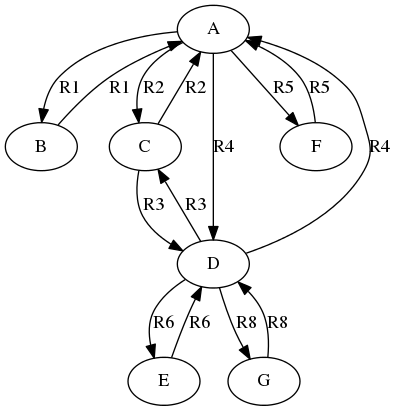
\includegraphics[height=5cm]{./png/GogolXL.png} }}%
  \qquad
  \subfloat[GogolXL with virtual edges]{{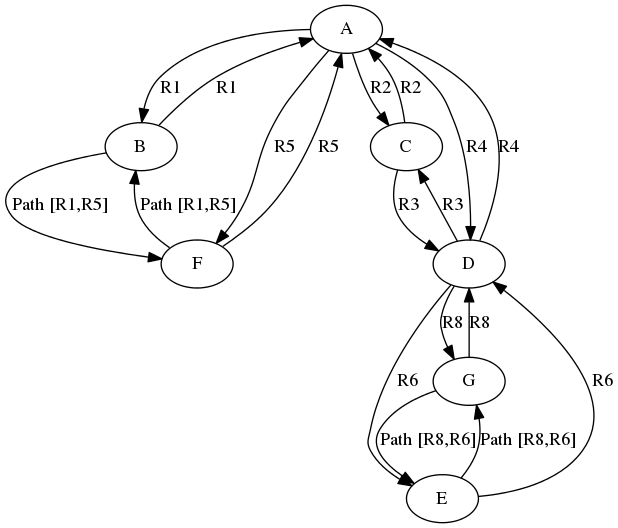
\includegraphics[height=7cm]{./png/XLLL.png} }}%
  \caption{Etat initial}%
  \label{fig:example}%
\end{figure}

\begin{figure}[h!]
  \centering
  \subfloat[Step 0]{{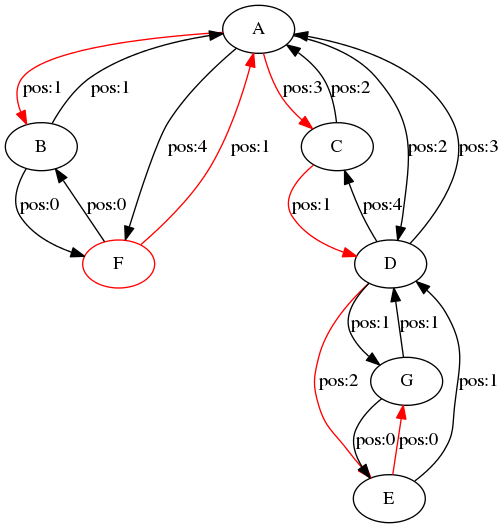
\includegraphics[height=7cm]{./png/GogolL_XLL_step_0.png} }}%
  \qquad
  \subfloat[Step 1]{{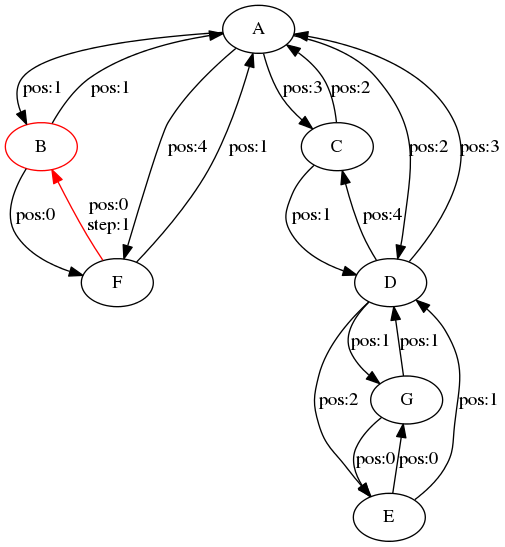
\includegraphics[height=7cm]{./png/GogolL_XLL_step_1.png} }}%
  
  \subfloat[Step 2]{{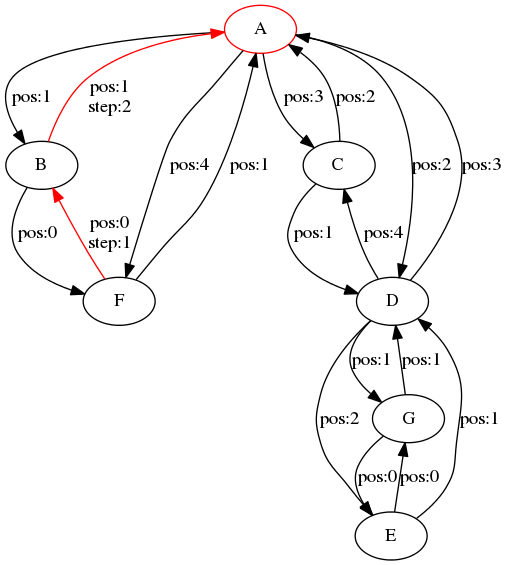
\includegraphics[height=7cm]{./png/GogolL_XLL_step_2.png} }}%
  \qquad
  \subfloat[Step 3]{{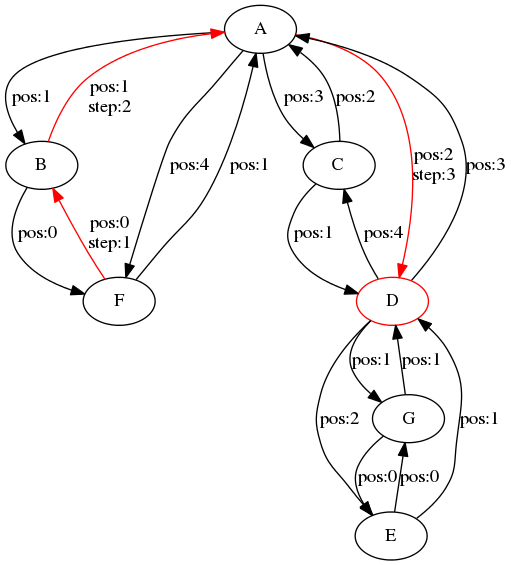
\includegraphics[height=7cm]{./png/GogolL_XLL_step_3.png} }}%
\end{figure}
  
\begin{figure}[h!]
 \centering
  \subfloat[Step 4]{{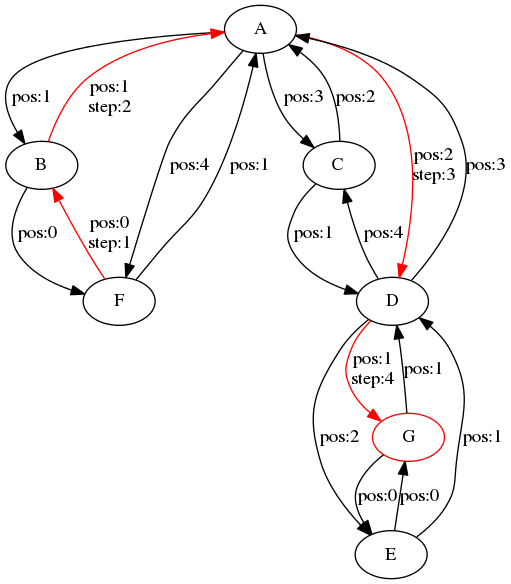
\includegraphics[height=7cm]{./png/GogolL_XLL_step_4.png} }}%
  \qquad
  \subfloat[Step 5]{{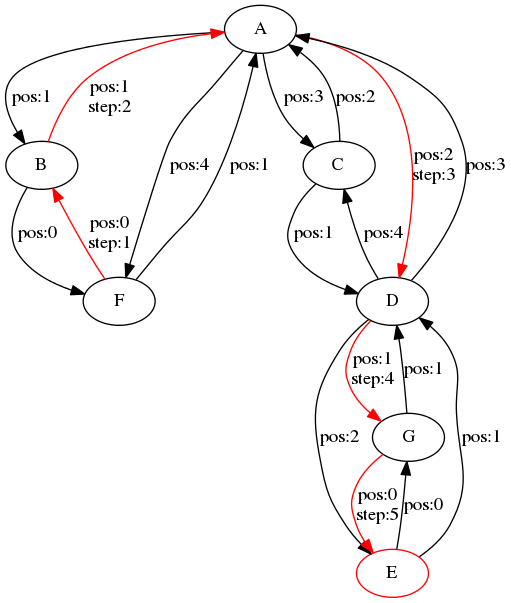
\includegraphics[height=7cm]{./png/GogolL_XLL_step_5.png} }}%
  
  \subfloat[Step 6]{{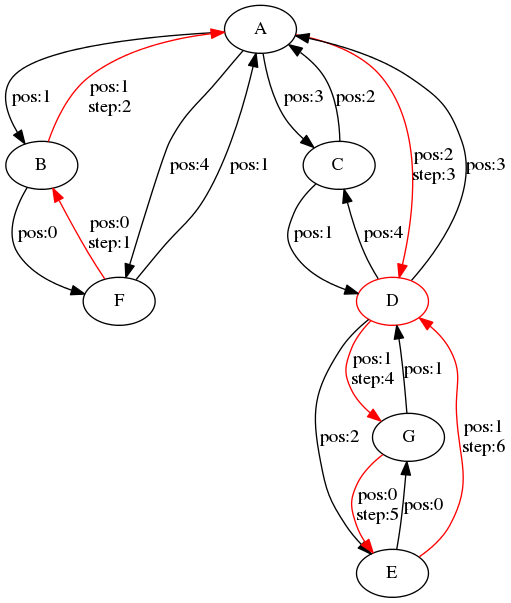
\includegraphics[height=7cm]{./png/GogolL_XLL_step_6.png} }}%
  \qquad
  \subfloat[Step 7]{{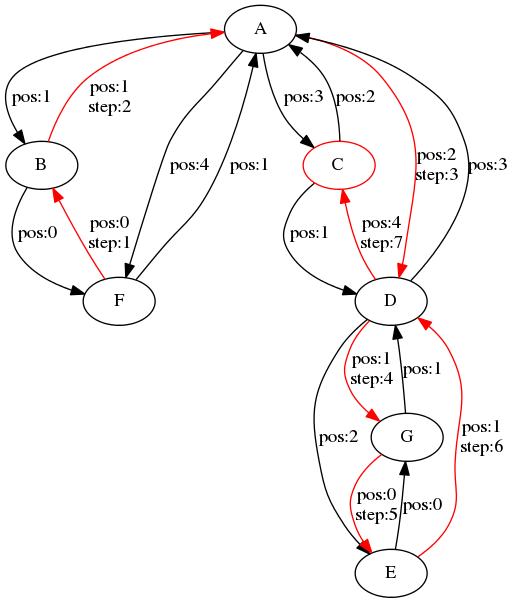
\includegraphics[height=7cm]{./png/GogolL_XLL_step_7.png} }}%

  \subfloat[Step 8]{{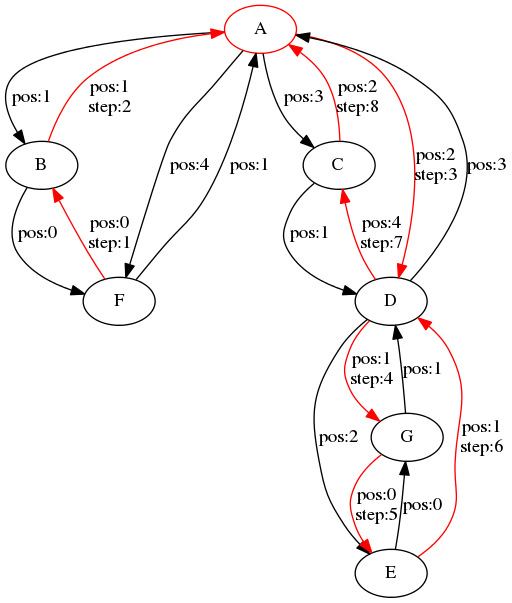
\includegraphics[height=7cm]{./png/GogolL_XLL_step_8.png} }}%
  \qquad
  \subfloat[Step 9]{{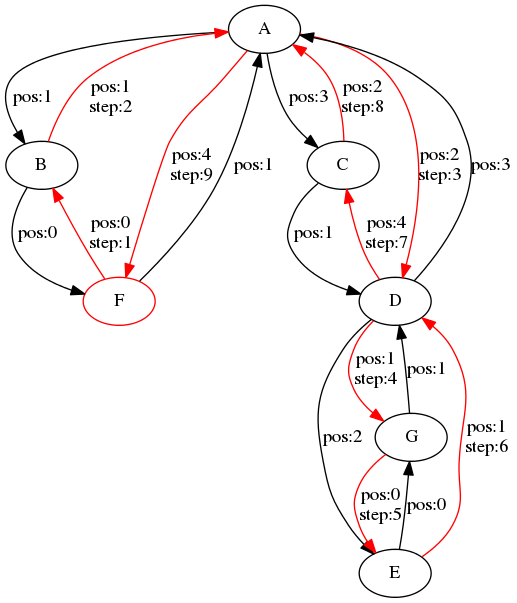
\includegraphics[height=7cm]{./png/GogolL_XLL_step_9.png} }}%
  
  \caption{Execution}%
  \label{fig:example}%
\end{figure}


\section*{Conclusion}
Stream API nous permet d’écrire ce que nous voulons obtenir sans préciser comment on souhaite l'obtenir. ce qui permet a la VM de construire elle même l’exécution la plus adapte.



\end{document}
